\documentclass{beamer}
\usetheme{Madrid}
\AtBeginSection[]{
  \begin{frame}
    \tableofcontents[currentsection]
  \end{frame}
}

\title{Prediction of Credit Card Default and Fraud using Machine Learning Techniques}
\subtitle{}
\author{Karthik, Pranjal, Rathi Saurabh, Vinay}
\institute{IIT(BHU), Varanasi}
\date{}


\setbeamertemplate{bibliography item}


\begin{document}
\begin{frame}
\titlepage
\end{frame}

\begin{frame}{
	\begin{center}Table Of Contents\end{center}}
\tableofcontents
\end{frame}
\section{Introduction}
\frame{
\frametitle{Introduction}
 \par  These days the amount of data collected in every field is very high, thus the need of applying Machine Learning to predict factors related to that field using the current data has become inevitable. In our research(exploratory) project, we chose to learn use existing Machine Learning Algorithms and try to suggest a new solution  to the problem of credit card default in banks. The main problem is to predict whether a new customer with few attributes will give back the money or default. This research work will be very useful for banks and in the finance sectors where loans and credit cards are given on a day to day basis.
}
\section{Data Sets}
\subsection{Data Set Introduction}
\frame{
\frametitle{Data Set  Introduction}
In our project, we have used two datasets. One being the details of customers of a bank in Taiwan which has 24 attributes like the amount of given credit, gender of the person, education, marital status, age and history of past payments. The dataset has 30000 instances and was collected in 2005.\par
  The second dataset consists of transactions made by credit cards in September 2013 by European credit card holders. There are over 284 thousand instances out of which 492 were frauds. The dataset consists of only numerical input variables which is a result of Principal Component Analysis and only two attributes could not be changed which are time and amount.
}
\subsection{Data Set Analysis}
\frame{
\frametitle{Data Analysis}
	\par The first dataset on analysis showed that approximately 70 \% data corresponds to non default transactions and 30\% corresponded to defaulted transations (shown in Fig 1). This is a bit skewed data but it can be neglected and our algorithms can be applied.\\
\begin{figure}
  \centering
  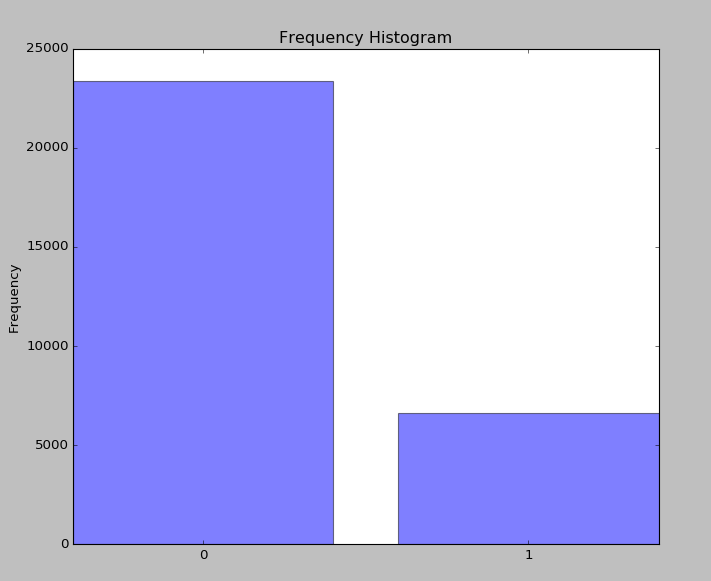
\includegraphics[scale=.2]{data1freq.png}
  \caption{Frequency Histogram of first data set}
  
\end{figure}
}
\frame{
\frametitle{Data Analysis}
	\par	The second dataset on the other hand was highly skewed with only 492 out of 2,84,000 being defaulted transactions. That amounts to .2\% of data being "1" and others being "0"(shown in Fig 2). This much skewedness had to be handled as just predicting "0" gives us an accuracy of 99.8\% but we have predicted all defaulted transations wrong which is a very big problem.
\begin{figure}
  \centering
  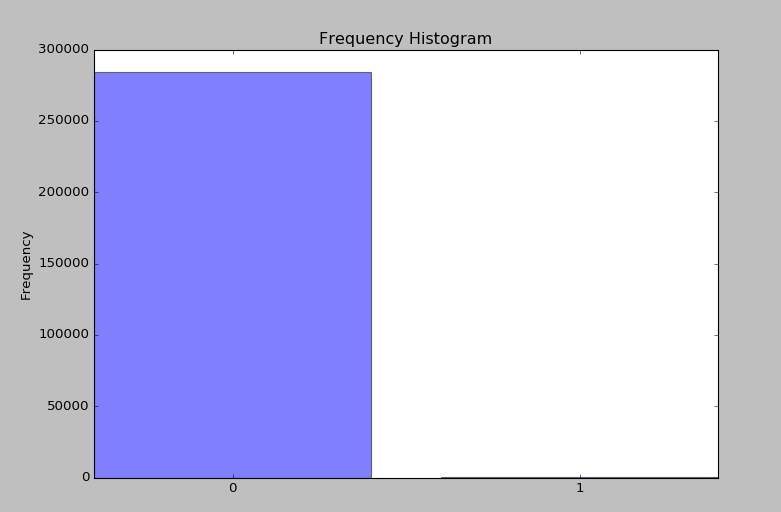
\includegraphics[scale=.2]{freq2init.png}
  \caption{Frequency Histogram of second data set before resampling}
  
\end{figure}
}
\frame{
\frametitle{Data Analysis}
	\par	To address this skewedness, we need to come up with few techniques. The technqiues which we can use to resample are
\begin{enumerate}
	\item Collecting more data (which is not possible now)
	\item Over-Sampling, which is adding copies of underrepresented class
	\item Under-Sampling, which is removing copies of overrepresented class
	\item SMOTE- Synthetic Minority Over-Sampling Technique which is a mixture of both Under and Over Sampling.
\end{enumerate}
}
\frame{
\frametitle{Data Analysis}
	\par We tried Under-Sampling wherein we randomly removed the "0"s and reduced the total instances to around 1350. Now the "1"s represented approximately 35\% of dataset [Refer Fig 3 for clearer analysis].
	\begin{figure}
  \centering
  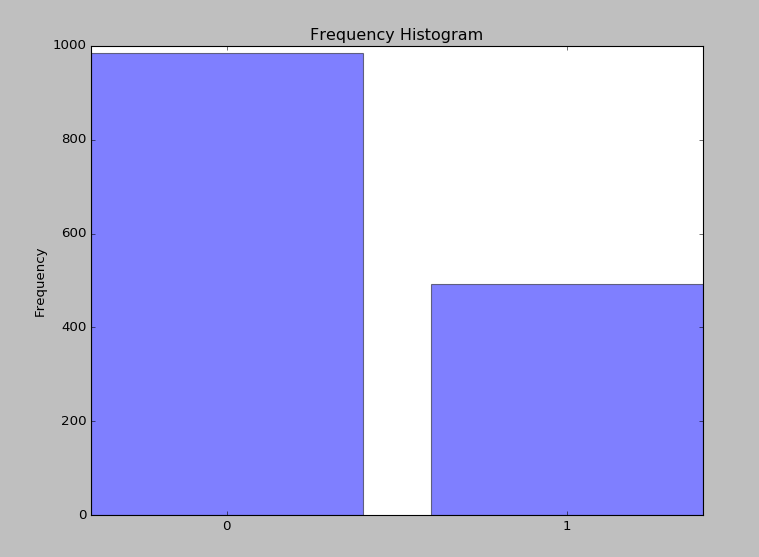
\includegraphics[scale=.18]{freq2fin.png}
  \caption{Frequency Histogram of second data set after resampling}
  
\end{figure}
}
\section{Machine Learning Techniques}
\subsection{Logistic Regression}
\frame{
\frametitle{Logistic Regression}
    \par In Machine Learning, logistic regression is a statistical method wherein we try to approximate the hypothesis by minimising the cost associated with the hypothesis.In this form of regressive analysis, we approximate the hypothesis to be a linear model of the features (independent variables). Logistic Regression is used for predicting binary dependent variables rather than a continuous outcome. Here in our project the binary dependent variable is that the credit has been defaulted or not. If not defaulted the binary variable is '0' else the binary variable is '1'.
    \par We assume Y to be a linear combination of the attributes.
    $p_{\theta}(x) = \Sigma \theta_{i}x_{i}$
    	Now in our classification problem $y$ can only be 1 or 0. So to correct the $y$, we introduce a Sigmoid function \begin{center}$q(x) = \frac{1}{1+e^{-x}}$ \end{center}. The speciality of the function is it's range is $[0,1]$ and with the value of 0.5 at $x=0$.
 Now is we replace  $p_{\theta}(x)$  as \begin{center}
 $p_{\theta}(x) = q(\theta^{T}x)$
 \end{center}
 }
 \frame{
 \frametitle{Logistic Regression}
 We initialise all $\theta_{i}$ to $0$ initially. Now let the cost function \begin{center}
 $W(y |x;\theta ) = (p_{\theta}(x))^{y}(1-p_{\theta}(x))^{1-y} $
 \end{center}.
	This function $W(y)$ tries to convey the difference between our prediction for the training data and the actual value. Now to fit the $\theta$ , we will maximise the likelihood \begin{center}
	$J(\theta)= \Pi_{i=1}^{m}  W(y |x;\theta) $ 
	\end{center}
  	We know it is better to maximise the log likelihood. Thus taking log \begin{center}
  	$log(B(\theta)) = \Sigma_{i=1}^{m} y^{(i)}log(p(x^{(i)})) + (1-y^{(i)})log(1-p(x^{(i)}))$
  	\end{center}
   To maximise the log likelihood, we use the \textbf{Gradient Descent} algorithm which is \\
   Repeat until convergence \{  \begin{center}
   $\theta_{j} := \theta_{j} + \alpha \frac{\partial log(B(\theta))}{\partial \theta_{j}}$ (for every $j$) \end{center}
   \} \\
}    
\subsection{Naive Bayesian}
\frame{
\frametitle{Naive Bayesian}
 It is a Machine Learning technique based on Bayes theorem with an assumption of independence among predictors. Naive Bayesian technique assumes that all the features are independent of each other. Bayes theorem mathematically implies\begin{center}
  $P(A|B) = \frac{P(B|A) P(A)}{P(B)}$
  \end{center}
  where \\
  $P(A|B)$ is the probability that event A occurs given event B\\
  $P(A)$ is the probability of occurence of event A\\
  $P(B)$ is the probability of occurence of event A\\
  $P(A|B)$ is the probability that event B occurs given event A\par
  The question now arises is how to calculate the probability?\par
  Now if the features take discrete values, we can then find the probability from the formula \begin{center}
  $P(A)= \frac{cnt(A)}{totalcnt}$
\end{center}
}
\frame{
\frametitle{Naive Bayesian}
 But if the data is continuous instead of discrete, we apply some standard probability functions. Here we will use Gaussian(Normal) Probability distribution function for the prediction of probability.\begin{center}
	$P(x) = \frac{1}{\sqrt{2\sigma^{2}\pi}}e^{\frac{(x-\mu)^{2}}{\sqrt{2}\sigma}}$
\end{center}
}
\subsection{Decision Trees}
\frame{
\frametitle{Decision Trees}
Decision trees build regression models based on a structure of the tree. In Machine Learning, the decision is about a single predictor (attributes). In this algorithm, the main concept is to choose an attribute and make decisions on that and distribute the dataset according to the decision. Then recursively on the distributed datasets apply decisions on the other attributes and finally we reach a point that the dataset becomes completely homogeneous in one category.
\par The task is tough because we don't know upon which attribute the first decision has to be taken. Thus we solve this greedily. Our final destination is smaller and more homogeneous datasets. Thus at every step, we will try to maximise the homogeneity of the resulting datasets.
}
\frame{
\frametitle{Decision Trees}
Here the measure of homogeneity mathematically is the entropy of the dataset. In order to increase the homogeneity, we need to reduce to entropy of the datasets. Thus we have entropy of a random variable $X$
\begin{center}
    $Entropy(X) = -\sum  P(x_{k})\log_2 P(x_{k}) $  
\end{center}
Thus we take the initial dataset, find it's entropy. Divide the dataset according to every attribute available and then find the resulting entropy. The attribute which results with the least entropy is then chosen and the dataset is divided accordingly. Then the datasets which are formed from the above said action are solved recursively.
}
\subsection{k-Nearest Neighbours}
\frame{
\frametitle{k-Nearest Neighbours}
    \par $K$-nearest neighbours is machine learning algorithm widely used for classification problems. As the name suggests, to classify an test example, we compute it's distance from all the training examples. And divide the distances into different sets corresponding to the set which training sample belongs. The set which has least sum of $k$ smallest distances will be the required classification for the sample.
Here
\begin{center}
	$distance_{j}^{2} = \Sigma_{i=1}^{m}( Train_{ij} - Test_{i} )^{2} $\\	
\end{center}
where $distance_{j}$ represents distance of test example with the $j^{th}$ training example.\\
$m$ represents the number of feautures in the dataset\\
$Train_{ij}$ represents $i^{th}$ feature of the $j^{th}$ training example\\
$Test_{i}$ represents $i^{th}$ feature of test example.
}
\subsection{Neural Networks}
\frame{
\frametitle{Neural Networks}
\begin{figure}
  \centering
  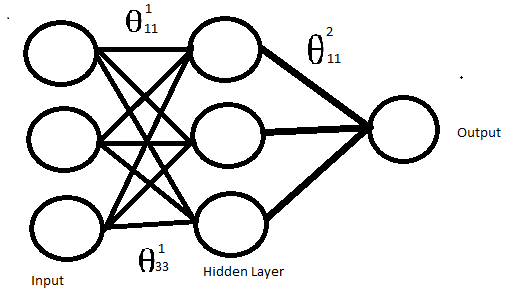
\includegraphics[scale=0.8]{Capture.png}
  \caption{Neural Networks}
\end{figure}
}
\frame{
\par Neural Networks is machine learning algorithm used for non-linear classification. In Neural Networks we consider hidden layers between input and output layer, for the each unit in the layer there is a mapping from each unit of previous layer having a particular weightage.
\par In this algorithm, we randomly initialise the mapping terms so called $\theta_{ij}^{l}$ terms ($l$ is the layer from which mapping is done, $i$ is the cell from which mapping is done and $j$ is the cell to which mapping is done in $(i+1)^{th}$ layer). Compute the terms in next layer and so on until the output layer. We calculate the cost function using the predicted output. The error in output helps in calculating errors from previous layer which further helps in calculating error from previous layers. These errors are used while calculating gradient of cost function with $\theta_{ij}^{l}$. Gradient Descent method is used to optimise cost function. In each such iteration of forward and backward propogation we improve the values of $\theta_{ij}^{l}$ and so the output.
}
\subsection{Support Vector Machines}
\frame{
\frametitle{Support Vector Machines}
	Support Vector Machines are supervised learning models which are used for binary classification.
    \begin{figure}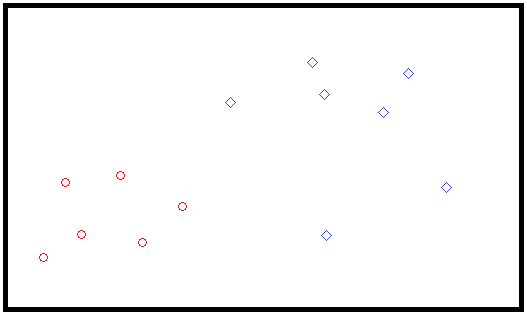
\includegraphics[scale=0.6]{Images/kachra.png}
			\caption{Positive Negative dataset}
			\end{figure}    
}
\frame{
    \begin{center}
        Hyperplanes
    \end{center}
    \begin{figure}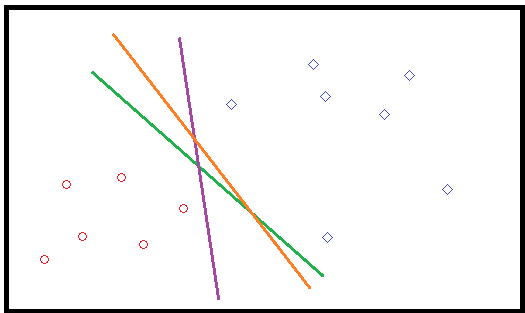
\includegraphics[scale=0.6]{Images/kachra1.png}
			\caption{Hyperplanes}
			\end{figure}
	Our task reduces to selecting best hyperplane.
}
\frame{
    \begin{center}
    Margin
    \end{center}

    \begin{figure}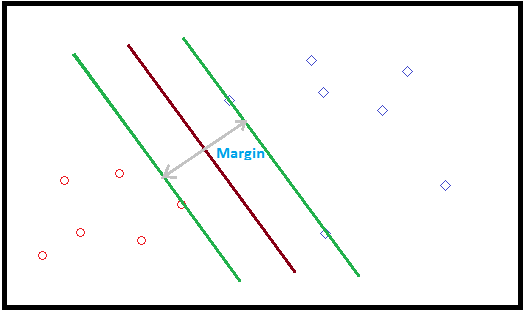
\includegraphics[scale=0.6]{Images/kachra2.png}
			\caption{Margin}
			\end{figure}
	Mathematically, hyperplane with highest margin gives best results.
}
\subsection{Proposed Technique}
\frame{
    \frametitle{
        Landmarks
    }
    \begin{figure}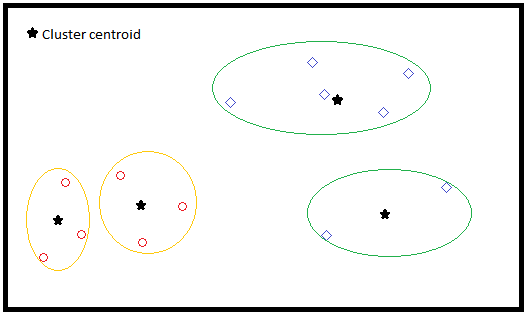
\includegraphics[scale=0.6]{Images/kachra3.png}
			\caption{Landmarks}
			\end{figure}
	Each cluster centroid functions as a special landmark.\\
	"Distances" from these landmarks can be treated as additional features.
}
\frame{
    We have considered the already given feature tuples as special points. That is, the values $X$s of a training data is a tuple, and we have $m$ such tuples because there are a total of $m$ training samples. 

Now in order to have more features, say $k$, we have applied k-means algorithm to find the centroids of $k$ clusters formed out of these tuples.

We have defined positive and negative clusters by having only positive points in positive cluster and negative points in negative cluster. We have proportionate number of positive and negative clusters to as there are number of positive and negative data points. 

These cluster centroids can now define the closeness of our given sample points.

This technique not only reduces the risk of underfitting by increasing the number of features, but also deals with the trouble of having a non-separable data in case of SVM.
SVM technique is supposed to be applied on linearly seperable data. This technique makes our data linearly seperable.
Although kernels can be used in case of SVM, this, infact, is a special case of kernels.

}
\section{Results}
\frame{
\frametitle{Plots}
\begin{figure}
  \centering
  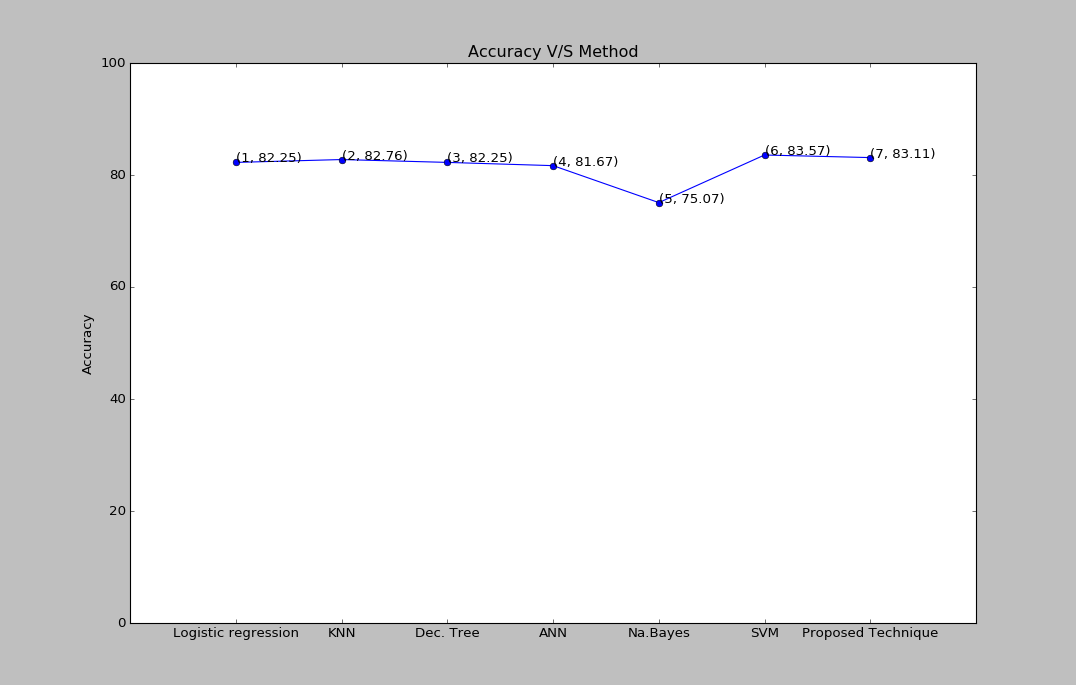
\includegraphics[scale=.25]{i1.png}
  \caption{Accuracies v/s Methods for Data set 1}  
\end{figure}
}
\frame{
\frametitle{Plots}
\begin{figure}
  \centering
  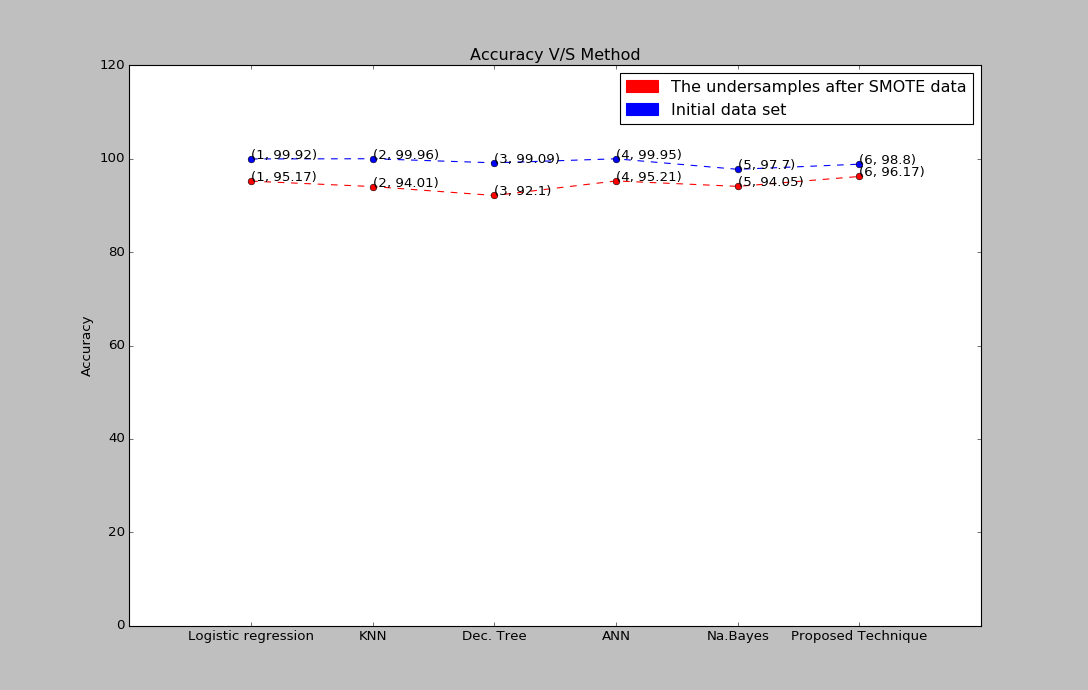
\includegraphics[scale=.25]{i2.png}
  \caption{Accuracies v/s Methods for Data set 2}  
\end{figure}
}
\frame{
\frametitle{Plots}
\begin{figure}
  \centering
  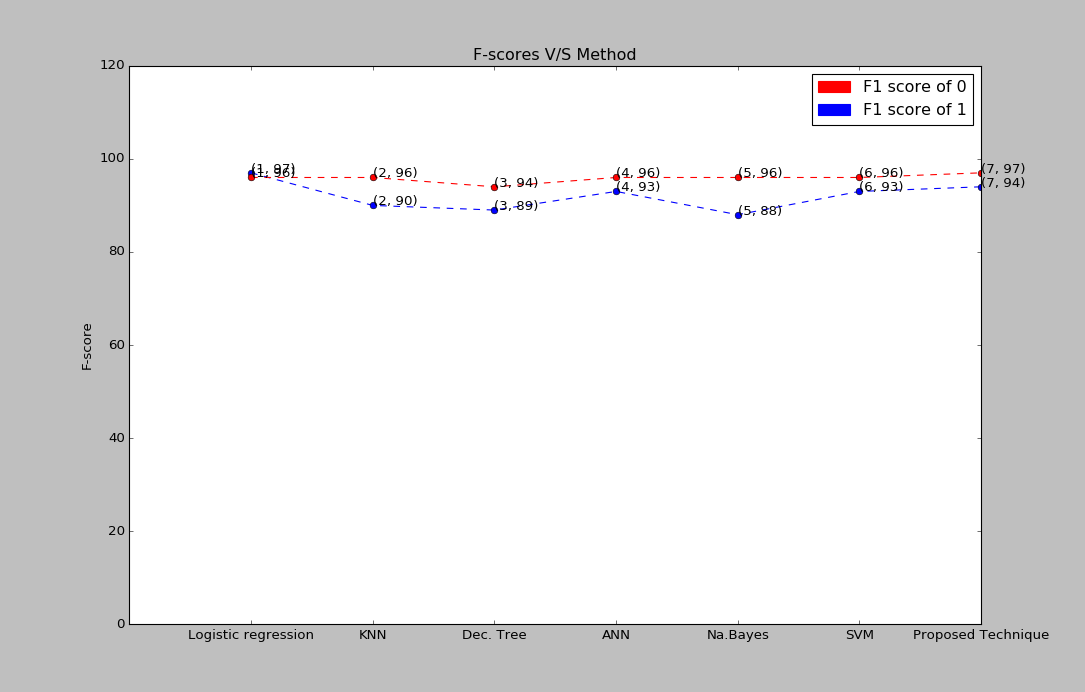
\includegraphics[scale=.25]{i3.png}
  \caption{F1- Scores of 0 and 1 after under-sampling}  
\end{figure}
}
\frame{
\frametitle{Plots}
\begin{figure}
  \centering
  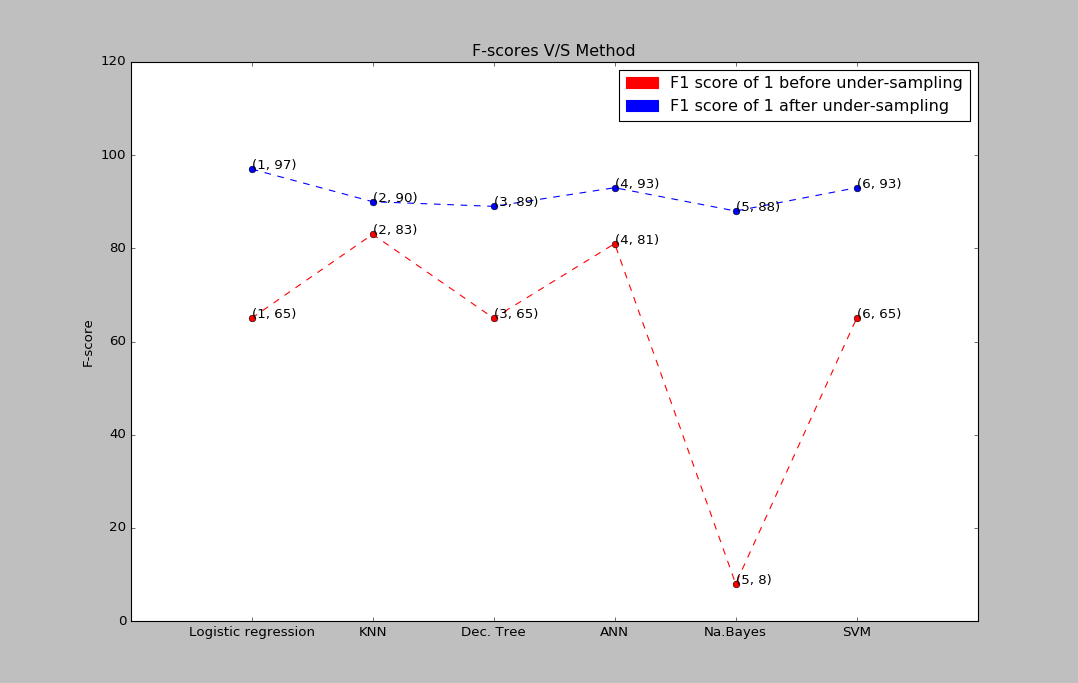
\includegraphics[scale=.25]{i4.png}
  \caption{F1- Scores of 1 before and after under-sampling}  
\end{figure}
}
\frame{
\frametitle{Conclusions}
This report gives rise to a number of important conclusions.
\begin{itemize}
\item In our first data set, we applied all techniques directly to the the given data and found SVM giving us the highest accuracy followed by our proposed methodology. The classification reports among all methods showed very less differences in the accuracies.
\item In the second data set, we applied the techniques before the re-sampling and found our models not predicting the ones properly. Thus some change had to be done in our model. Thus we under-sampled the data and drastically reduced the data set's size to 1300 and then we applied our machine learning techniques.\end{itemize}
}
\frame{
\begin{itemize}
\item After under-sampling, the overall results were lesser than that of the initial data set but the accuracy and $f1$ score of predicting 1 increased a lot and thus increasing the quality of our models.
\item Again in this data set, our proposed technique of applying K-means with SVM performs slightly better than other techniques.
\item Thus in our report, we applied all machine learning techniques and then compared them to find the best for the data sets.
\end{itemize}
}
\begin{frame}{}
	\centering \huge
	\emph{Thank You}
	
\end{frame}


\end{document}
